\documentclass[11pt,compress,final]{beamer}

\RequirePackage[english]{babel}
\RequirePackage{amsfonts,amssymb,amsmath,mathtools}
\RequirePackage[utf8]{inputenc}
\RequirePackage[T1]{fontenc}
\RequirePackage{lmodern}
\RequirePackage{mathpazo}
\usepackage{tikz}

\definecolor{LHCblue}{RGB}{10, 73, 132}
\usecolortheme[named=LHCblue]{structure}
\usepackage[bars]{beamerthemetree} %Beamer theme v 2.2
\usefonttheme[onlymath]{serif}
%\usepackage{kerkis}
\setbeamercovered{highly dynamic}
\usetheme{Ilmenau} % Beamer theme v 3.0
\useoutertheme[subsection=true]{smoothbars}%Beamer Outer Theme-circles on top
\usefonttheme{serif}
\useinnertheme{circles} %rectangle bullet points instead of circle ones
\usepackage{beamerthemebars}

\setbeamerfont{section in toc}{size=\small}
\setbeamerfont{subsection in toc}{size=\small}
\setbeamercolor{subsection in toc}{fg=LHCblue!40!black}
\expandafter\def\expandafter\insertshorttitle\expandafter{%
  \insertshorttitle\hfill%
  \insertframenumber\,/\,\inserttotalframenumber}
\setbeamertemplate{navigation symbols}{}%remove navigation symbols

\AtBeginSection[]
{
  \begin{frame}
  \frametitle{Plan}
  \begin{columns}[t]
  \begin{column}{5cm}
  \tableofcontents[sections={1-3},currentsection, hideothersubsections]
  \end{column}
  \begin{column}{5cm}
  \tableofcontents[sections={4-6},currentsection,hideothersubsections]
  \end{column}
  \end{columns}
  \end{frame}
}

\author{Clément PARISOT}
\title{Young engineers seminar}
\subtitle{Grid'5000 support and services orchestration}
\institute{IJD INRIA Nancy\\MADYNES Team\vspace{2.75cm}}
\begin{document}
\titlegraphic{%
\begin{center}

\includegraphics[height=1.25cm]{figures/inria-logo}
\hspace{30mm}

\includegraphics[height=1.25cm]{figures/g5k-logo}
\end{center}
}
\date{\scriptsize \today}

{
\setbeamertemplate{footline}{} 
\setbeamertemplate{headline}{}
\usebackgroundtemplate{
  \begin{tikzpicture}
    \path [outer color = LHCblue!15, inner color = white]
      (0,0) rectangle (\paperwidth,\paperheight);
  \end{tikzpicture}}
\begin{frame}[plain]
  \titlepage
\end{frame}
}
\addtocounter{framenumber}{-1}
\institute{IJD INRIA Nancy}

\begin{frame}
\frametitle{Summary}
\begin{columns}[t]
  \begin{column}{5cm}
  \tableofcontents[sections={1-3},hideothersubsections]
  \end{column}
  \begin{column}{5cm}
  \tableofcontents[sections={4-6},hideothersubsections]
  \end{column}
  \end{columns}
\end{frame}

\section{Introduction}
\subsection{Grid'5000}
\begin{frame}
\frametitle{Grid'5000 platform}
\begin{block}{}
\textbf{Grid'5000}: a large-scale and versatile distributed testbed for experiments-driven research on parallel and distributed systems
\end{block}
\begin{itemize}
\item Created in 2003
\item Bare metal ressources
\item Give users root access to the compute nodes
\item Deploy environment (kadeploy)
\item Network configuration (kavlan)
\item Allows experiments on all the software layers
\end{itemize}
\end{frame}

\begin{frame}
\frametitle{Grid'5000 today (2016/11)}
\begin{columns}[c]
  \begin{column}{6cm}
	\begin{itemize}
	\item 7 sites in France
	\item 1 site in Luxembourg
	\item 10G dedicated Renater network
	\item 30 clusters
	\item 903 nodes
	\item 8700 cores
	\item 84 accelerators (Xeon Phi/GPU)
	\item 1076 users over the last 3 years
	\end{itemize}
  \end{column}
  \begin{column}{6cm}
	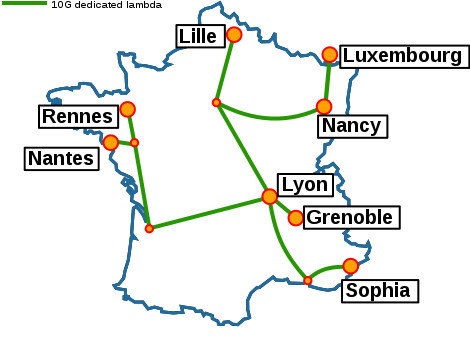
\includegraphics[scale=0.42]{figures/Renater5-g5k}
  \end{column}
\end{columns}
\end{frame}

\begin{frame}
\frametitle{Grid'5000 today (2016/11)}
\begin{center}
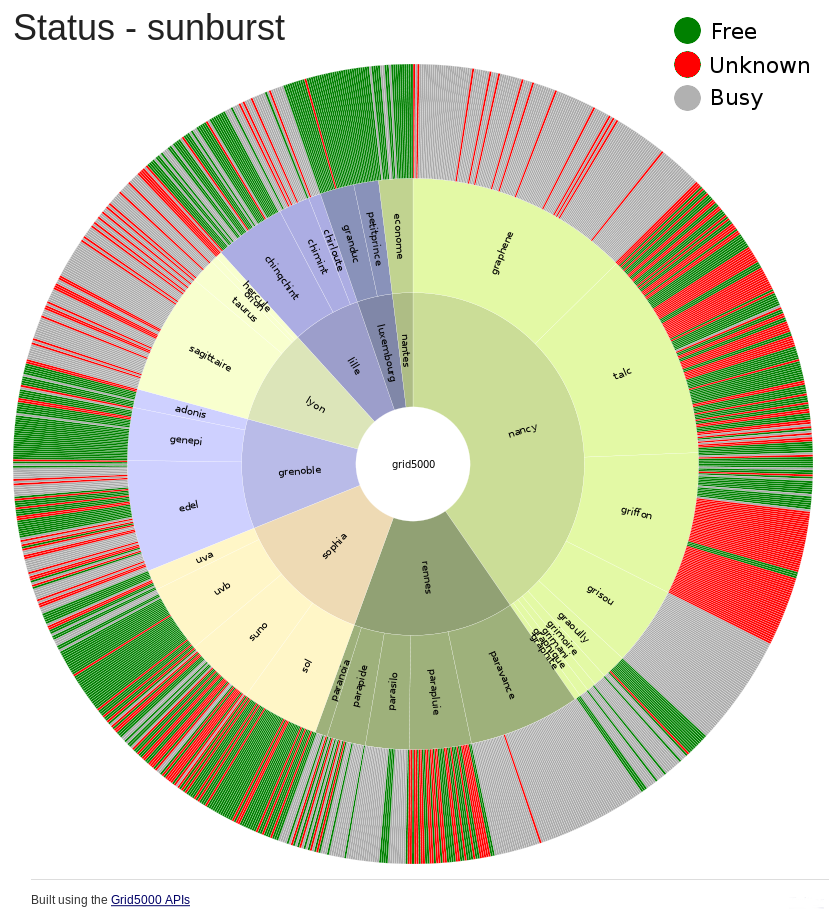
\includegraphics[scale=0.19]{figures/sunburst}
\end{center}
\end{frame}

\section{Support}
\subsection{Admin job}
\begin{frame}
\frametitle{Support team tasks}
Day-to-Day Tasks
\begin{itemize}
\item Weekly phone meeting
\item Answering users mails
\item System administration
\item Network administration
\item Grid'5000 tools improvement
\end{itemize}
Background Tasks
\begin{itemize}
\item Kwapi: energy and network monitoring tool
\item Production jobs integration in Grid'5000
\item Integration of 6 new clusters
\item Storage addition in Talc
\item Backup /home directories of local users
\end{itemize}
\end{frame}


\subsection{Monitoring services and alerts}
\begin{frame}
\frametitle{Nagios dashboard}
\begin{center}
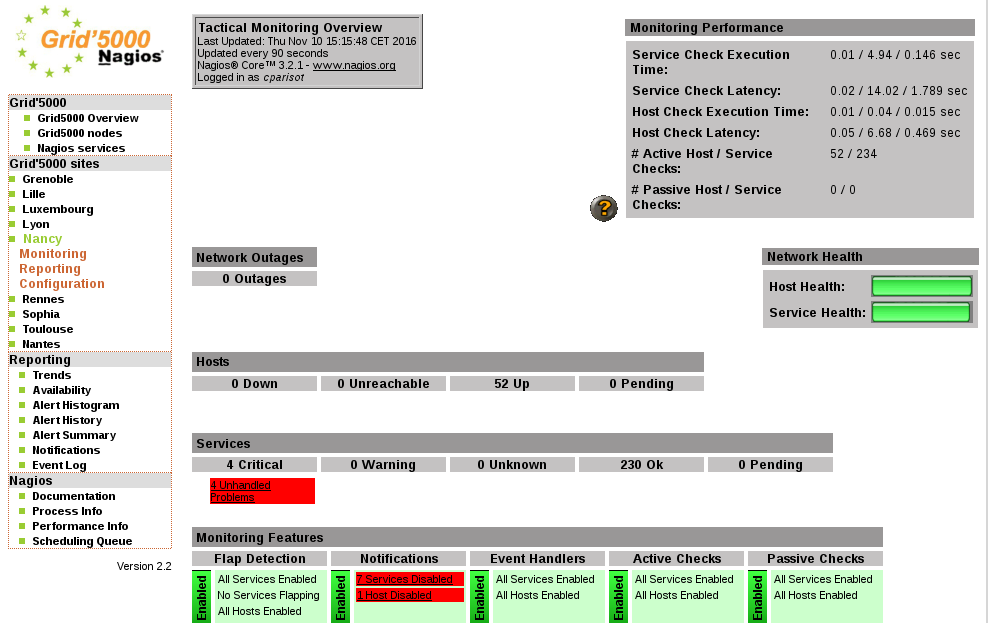
\includegraphics[scale=0.29]{figures/nagios}
\end{center}
\end{frame}

\begin{frame}
\frametitle{Nagios overview}
\begin{itemize}
\item Monitoring of the infrastructure
\item Alerts on load, ping, Hard disk failure, ...
\item One server per site
\item Reporting by mail 
\end{itemize}
\end{frame}

\begin{frame}
\frametitle{Icinga dashboard}
\begin{center}
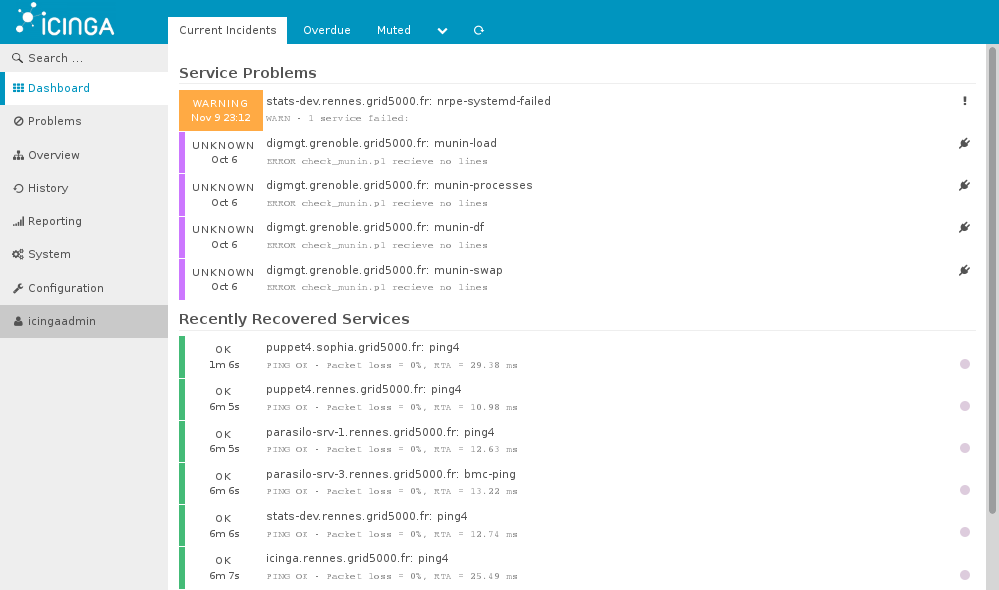
\includegraphics[scale=0.30]{figures/icinga}
\end{center}
\end{frame}

\begin{frame}
\frametitle{Icinga overview}
\begin{itemize}
\item Better UI
\item Unified dashboard for global view
\item Compatibility with Nagios (old) checks
\item Distributed monitoring
\end{itemize}
\begin{center}
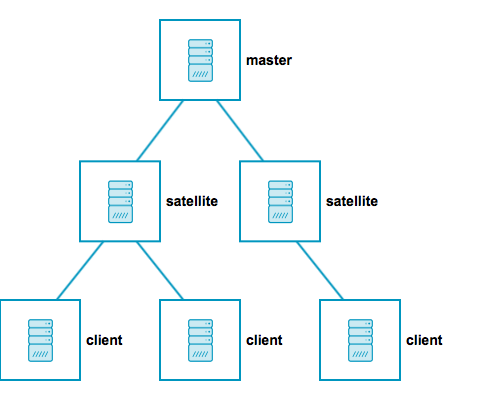
\includegraphics[scale=0.3]{figures/icinga2_distributed_roles}
\end{center}
\end{frame}

\subsection{Incident and ticket}
\begin{frame}
\frametitle{Bugzilla: different sorts of ticket}
\begin{itemize}
\item Incident reaction (network broken, services down...)
\item Event on Grid'5000 (maintenance, update...)
\item Problem with a node, environment or software
\item Feature request
\item Daily tasks (project management)
\end{itemize}
\end{frame}

\begin{frame}
\frametitle{Bugzilla: how to fill a ticket}
%\begin{columns}[c]
%  \begin{column}{4cm}
%\begin{tiny}
%\begin{enumerate}
%\item[Component:] a site, an internal/external service, network, documentation ?
%\item[Severity:] high, medium, low, to discuss
%\item[Assignee:] person in charge of the resolution
%\item[Status:] New, Assigned, Resolved
%\item[Keywords:] event, incident, task of a project
%\end{enumerate}
%\end{tiny}
%\end{column}
%  \begin{column}{6cm}
  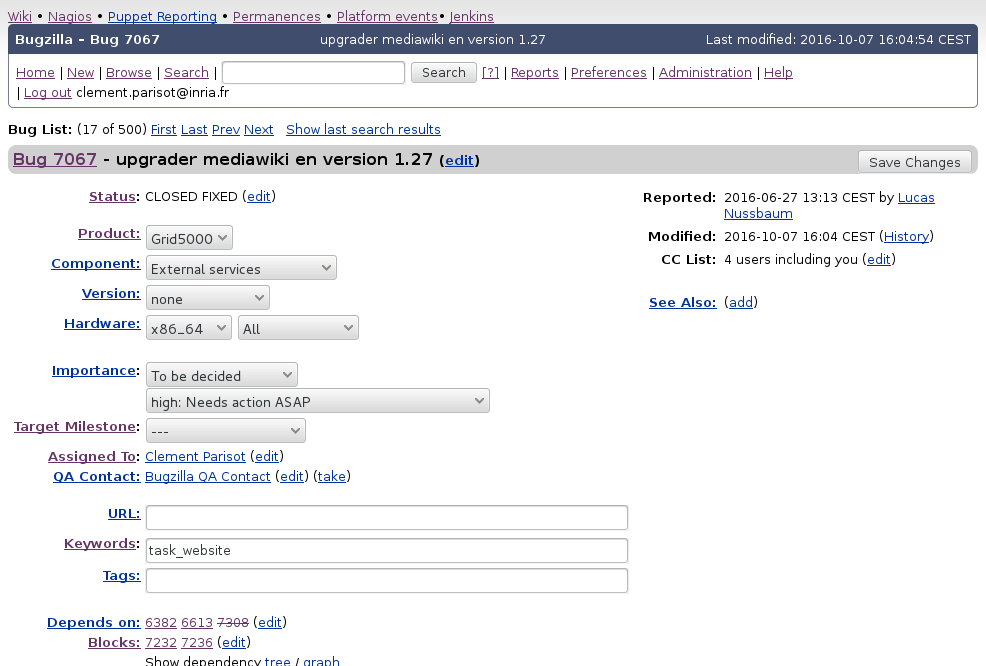
\includegraphics[scale=0.29]{figures/bugzilla_ticket}
%  \end{column}
%\end{columns}
\end{frame}

\section{Services orchestration}
\subsection{Xen/Puppet4}
\begin{frame}
\frametitle{Virtualisation of services infrastructure with Xen}
\begin{center}

\includegraphics[scale=0.04]{figures/xen}
\end{center}
\begin{itemize}
\item 1 VM (domU) for each service
\begin{itemize}
\item Supervision
\item DNS
\item mediawiki
\end{itemize}
\item 1 to 3 hypervisor (dom0) per site
\item Filesystem: lvm and ext4
\item OS: Debian (lenny, squeeze, wheezy and jessie)
\item No manager to create, destroy or migrate the VM (Xen CLI) 
\end{itemize}
\end{frame}

\begin{frame}
\frametitle{Puppet for services management}
\begin{center}

\includegraphics[scale=0.2]{figures/puppet}
\end{center}
\begin{columns}
\begin{column}{8cm}
\begin{itemize}
\item Configuration management
\item Model-driven approach
\item 1 module for each application (nagios, bugzilla, apache, ...)
\item Puppet run on all the VM and configure:
\begin{itemize}
\item Files (content, owner, rights...)
\item Packages (present, absent, version, ...)
\item Services (running, stopped)
\end{itemize}
\end{itemize}
\end{column}
\begin{column}{3cm}

\includegraphics[scale=0.15]{figures/puppet_config}
\end{column}
\end{columns}
\end{frame}

\section{Example: Mediawiki upgrade}
\subsection{Package creation}
\begin{frame}
\frametitle{How to upgrade mediawiki}
\begin{center}

\includegraphics[scale=0.2]{figures/mw}
\end{center}
\begin{block}{Procedure}
\begin{enumerate}
\item Upgrade version of: mysql, php
\item Read release notes
\item Dump existing DB files (backup)
\item Upload tarball and untar
\item Adapt LocalSettings.php file
\item Change rights/owner on images directory
\item Run the upgrade script
\end{enumerate}
\end{block}
\end{frame}

\begin{frame}
\frametitle{Create a Debian package for mediawiki}
\begin{center}

\includegraphics[scale=0.3]{figures/deb_package}
\end{center}
\begin{itemize}
\item Untar the mediawiki to the correct location
\item Just add dependances to packages and their versions in the debian control file
\item Add a postinstall script to change the right/owner on images directory
\item Eventually run the upgrade script at the end
\item Specify the version installed by this package
\end{itemize}
\begin{block}{}
Debian will manage the dependances of packages and their version for us
\end{block}
\end{frame}

\subsection{Vagrant}
\begin{frame}
\frametitle{Testing environment}
\begin{center}

\includegraphics[scale=0.15]{figures/vagrant}
\end{center}
\begin{block}{}
Create and configure lightweight, reproducible, and portable development environments.
\end{block}
\begin{itemize}
\item Single file to describe the type of machine you want
\begin{itemize}
\item OS (Debian)
\item Software installed (Puppet)
\item Host file sharing
\item Network binding (access to Grid'5000 API)
\end{itemize}
\item Single command to create the development environment
\begin{itemize}
\item vagrant up
\end{itemize}
\end{itemize}
\end{frame}

\begin{frame}
\frametitle{Test Puppet execution in Vagrant}
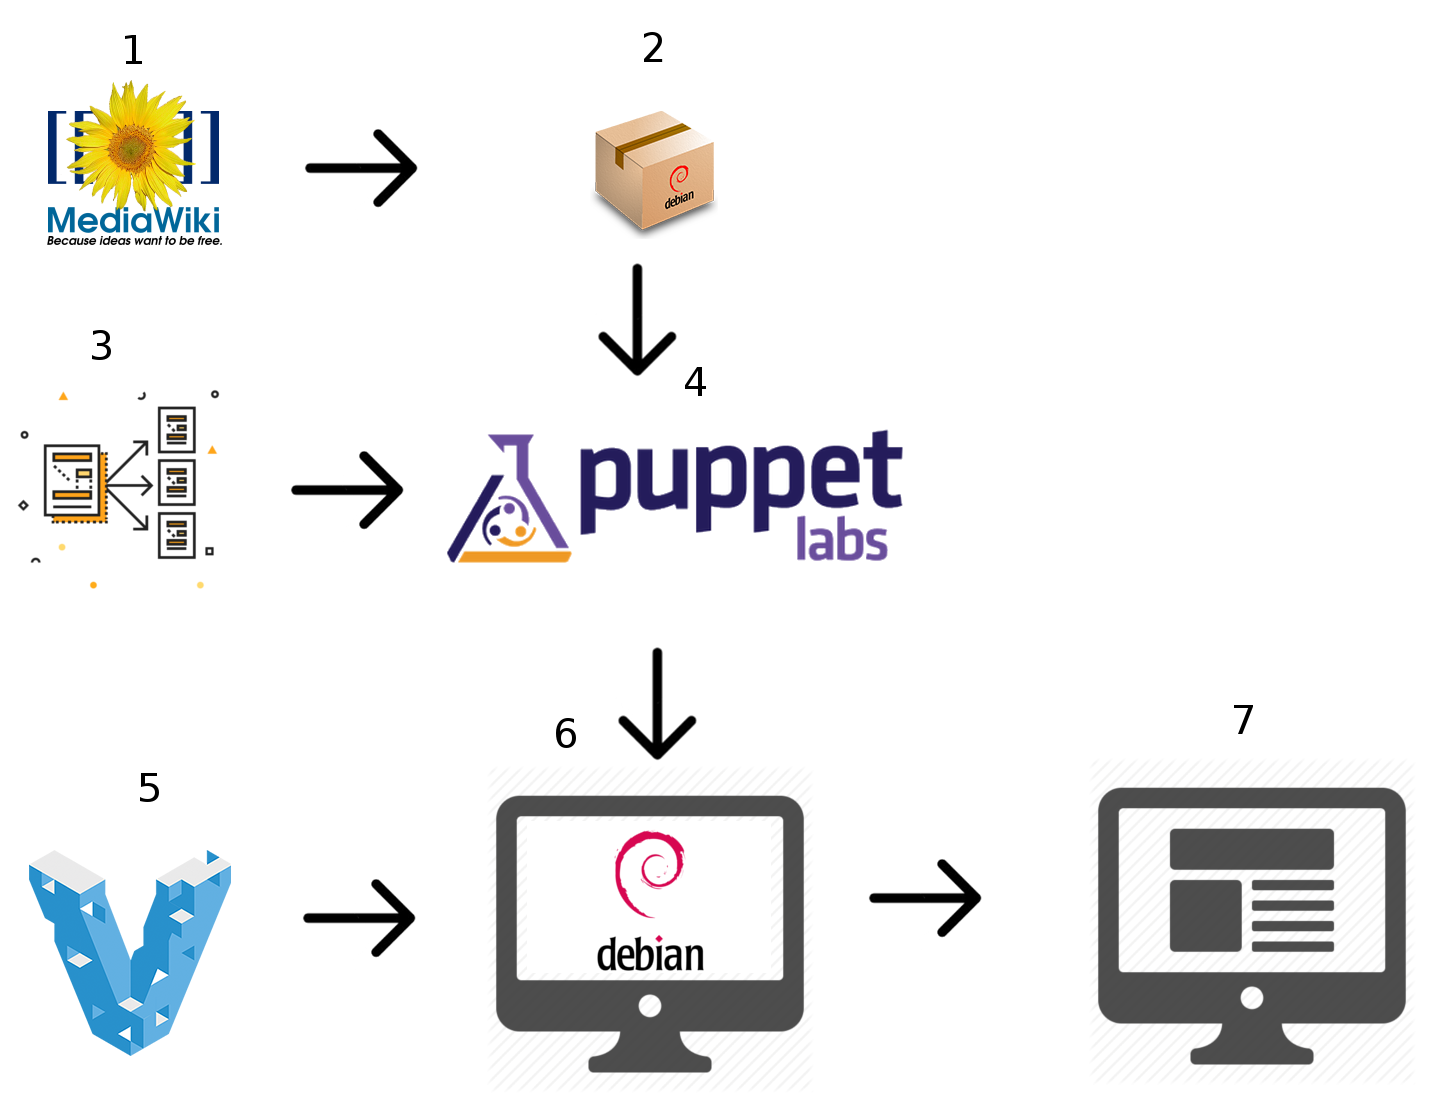
\includegraphics[scale=0.16]{figures/process}
\end{frame}

\begin{frame}
\frametitle{Test Puppet execution in Vagrant}
\begin{block}{Local test: laptop}
\begin{itemize}
\item Create the mediawiki Puppet module which install mediawiki package
\item Create a Vagrantfile for a Debian+Puppet environment
\item Dump the actual wiki database and use it in vagrant
\item Create a tunnel to the user and Grid'5000 API to test specific 'Special Pages'
\end{itemize}
\end{block}
At this point:
\begin{itemize}
\item \textbf{packaging problem} are removed
\item receipe works with the \textbf{production database}
\item \textbf{connection to API} is functionnal
\end{itemize}
\end{frame}

\subsection{Upgrade in production}
\begin{frame}
\frametitle{Tests in production}
\begin{block}{Nancy test: mediawiki-dev.nancy.grid5000.fr}
\begin{itemize}
\item Create a Xen+Puppet VM on Grid'5000 Nancy 
\item Run puppet on it
\item New problems apears:
\begin{itemize}
\item Connection inside of Grid'5000
\item Test of redirection with apache
\end{itemize}
\end{itemize}
\end{block}
At this point:
\begin{itemize}
\item \textbf{Grid'5000 puppet} can configure the VM
\item Connection with \textbf{Grid'5000 services} can be tested (nagios, syslogs, ...)
\end{itemize}
\end{frame}

\begin{frame}
\frametitle{Tests in production}
\begin{block}{Grid'5000: mediawiki.grid5000.fr}
\begin{itemize}
\item Test in DMZ
\item Last problems
\begin{itemize}
\item Filter rules on DMZ
\item Manual installed files (mediawiki plugins, themes)
\end{itemize}
\end{itemize}
\end{block}
At this point:
\begin{itemize}
\item Connection from \textbf{outside} of Grid'5000
\item Specific \textbf{security} rules
\end{itemize}
\end{frame}

\section{Conclusion}
\begin{frame}
\frametitle{Conclusion}
\begin{itemize}
\item Grid'5000 support team
\begin{itemize}
\item Lot of experience in system administration
\end{itemize}
\item Service orchestration
\begin{itemize}
\item Rebuild a service from scratch
\item Write a receipe and let puppet master play
\end{itemize}
\item Vagrant as an environment
\begin{itemize}
\item Reproducible
\item Shareable
\item 1 file and 1 command to test your receipes
\end{itemize}
\end{itemize}
\end{frame}

\section*{}
\begin{frame}
\frametitle{Sources}
\begin{scriptsize}
\begin{description}
\item[Grid'5000:]\url{https://grid5000.fr/}
\item[Nagios:]\url{https://www.nagios.org/}
\item[Icinga:]\url{https://www.icinga.org/}
\item[Bugzilla:]\url{https://www.bugzilla.org/}
\item[Puppet:]\url{https://puppet.com/}
\item[Vagrant:]\url{https://www.vagrantup.com/}
\item[Mediawiki-Vagrant:]\url{https://www.mediawiki.org/wiki/MediaWiki-Vagrant/fr}
\item[Mediawiki:]\url{https://www.mediawiki.org/wiki/MediaWiki}
\end{description}
\end{scriptsize}
\end{frame}
\end{document}
